\section{Basic}
	\subsection{vimrc}
			\lstinputlisting{Basic/vimrc}
	\subsection{Python stress}
			\lstinputlisting{Basic/stress/py.py}	
	
	\subsection{C++ stress}
			\lstinputlisting{Basic/stress/cpp.cpp}	
\newpage			
\section{Graph}
	\subsection{DSU}
		\lstinputlisting{Graph/DSU.cpp}
	\subsection{LCA}
		\lstinputlisting{Graph/LCA.cpp}
	\subsection{Dijkstra}
		\lstinputlisting{Graph/Dijkstra.cpp}

\section{Flow}
	\subsection{Dinic}
		\lstinputlisting{Graph/Flow/dinic.cpp}
	\subsection{MinCostFlow}
		\lstinputlisting{Graph/Flow/MinCostFlow.cpp}
		
\section{Matching}
	\subsection{KM}
		\lstinputlisting{Graph/Matching/Kuhn_Munkres.cpp}
		
\section{Geometry}
		\subsection{ConvexHull}
		\lstinputlisting{Geometry/Convex_Hull.cpp}

\section{Tree}
		\subsection{Trie}
		\lstinputlisting{Tree/Trie.cpp}
				
\section{Math}
		\subsection{Miller Rabin}
		\lstinputlisting{Math/Miller_Rabin.cpp}
		\subsection{Josephus Problem}
		\lstinputlisting{Math/Josephus_Problem.cpp}
		\subsection{Phi}
		\lstinputlisting{Math/Phi.cpp}
		\subsection{ChineseRemainder}
		\lstinputlisting{Math/chineseRemainder.cpp}
		\subsection{O(1)mul}
		\lstinputlisting{math/O(1)mul.cpp}
		\newpage
		\subsection{Pollard Rho}
		\lstinputlisting{math/pollardRho.cpp}
\section{Data Structure}
		\subsection{區間修改線段樹}
		\lstinputlisting{DataStructure/segmentTree_segmentModify.cpp}
		\newpage
		\subsection{pbdsKth}
		總共有$n$件衣服,各自有不同的價格$(a_1, a_2, ..., a_n)$。\\
一開始第$i$件會在編號為$i$的桶子裡,接下來會有$m$筆操作\\
每次操作有三種選擇:\\
- A x y :將編號第$x$的衣服所在桶子裡面所有的衣服,倒到第$y$件衣服所在的桶子 $(1 ≤ x, y ≤ n)$\\
- M x y :第$x$件衣服的售價改為$y (1 ≤ x ≤ n, 1 ≤ y ≤ 10^9)$\\
- Q x y :查詢第$x$件衣服所在的桶子,裡面第$y$大的售價 $(1 ≤ x ≤ n)$\\
\\
$1 ≤ n ≤ 10^5$\\
$1 ≤ m ≤ 4 * 10^5$\\
\\
5 4\\
7 8 5 13 12\\
Q 4 1\\
A 5 4\\
A 3 4\\
Q 4 3\\
\\
13\\
5\\
		\lstinputlisting{DataStructure/pbds_kth.cpp}
\newpage		
\section{Other}
		\subsection{Suifeng0214}
		\lstinputlisting{Other/suifeng0214.cpp}
		\subsection{Xiang1078}
		\lstinputlisting{Other/xiang1078.cpp}
		\newpage
		\subsection{jenny20030314}
		\lstinputlisting{Other/jenny20030314.cpp}
		\newpage
		\subsection{int128}
		\lstinputlisting{Other/int128.cpp}
		\newpage
		\subsection{Primes}
		\lstinputlisting{Other/primes.cpp}
		\newpage
		\subsection{Python cheatsheet}
		\lstinputlisting{Other/python.py}
\onecolumn
\centering
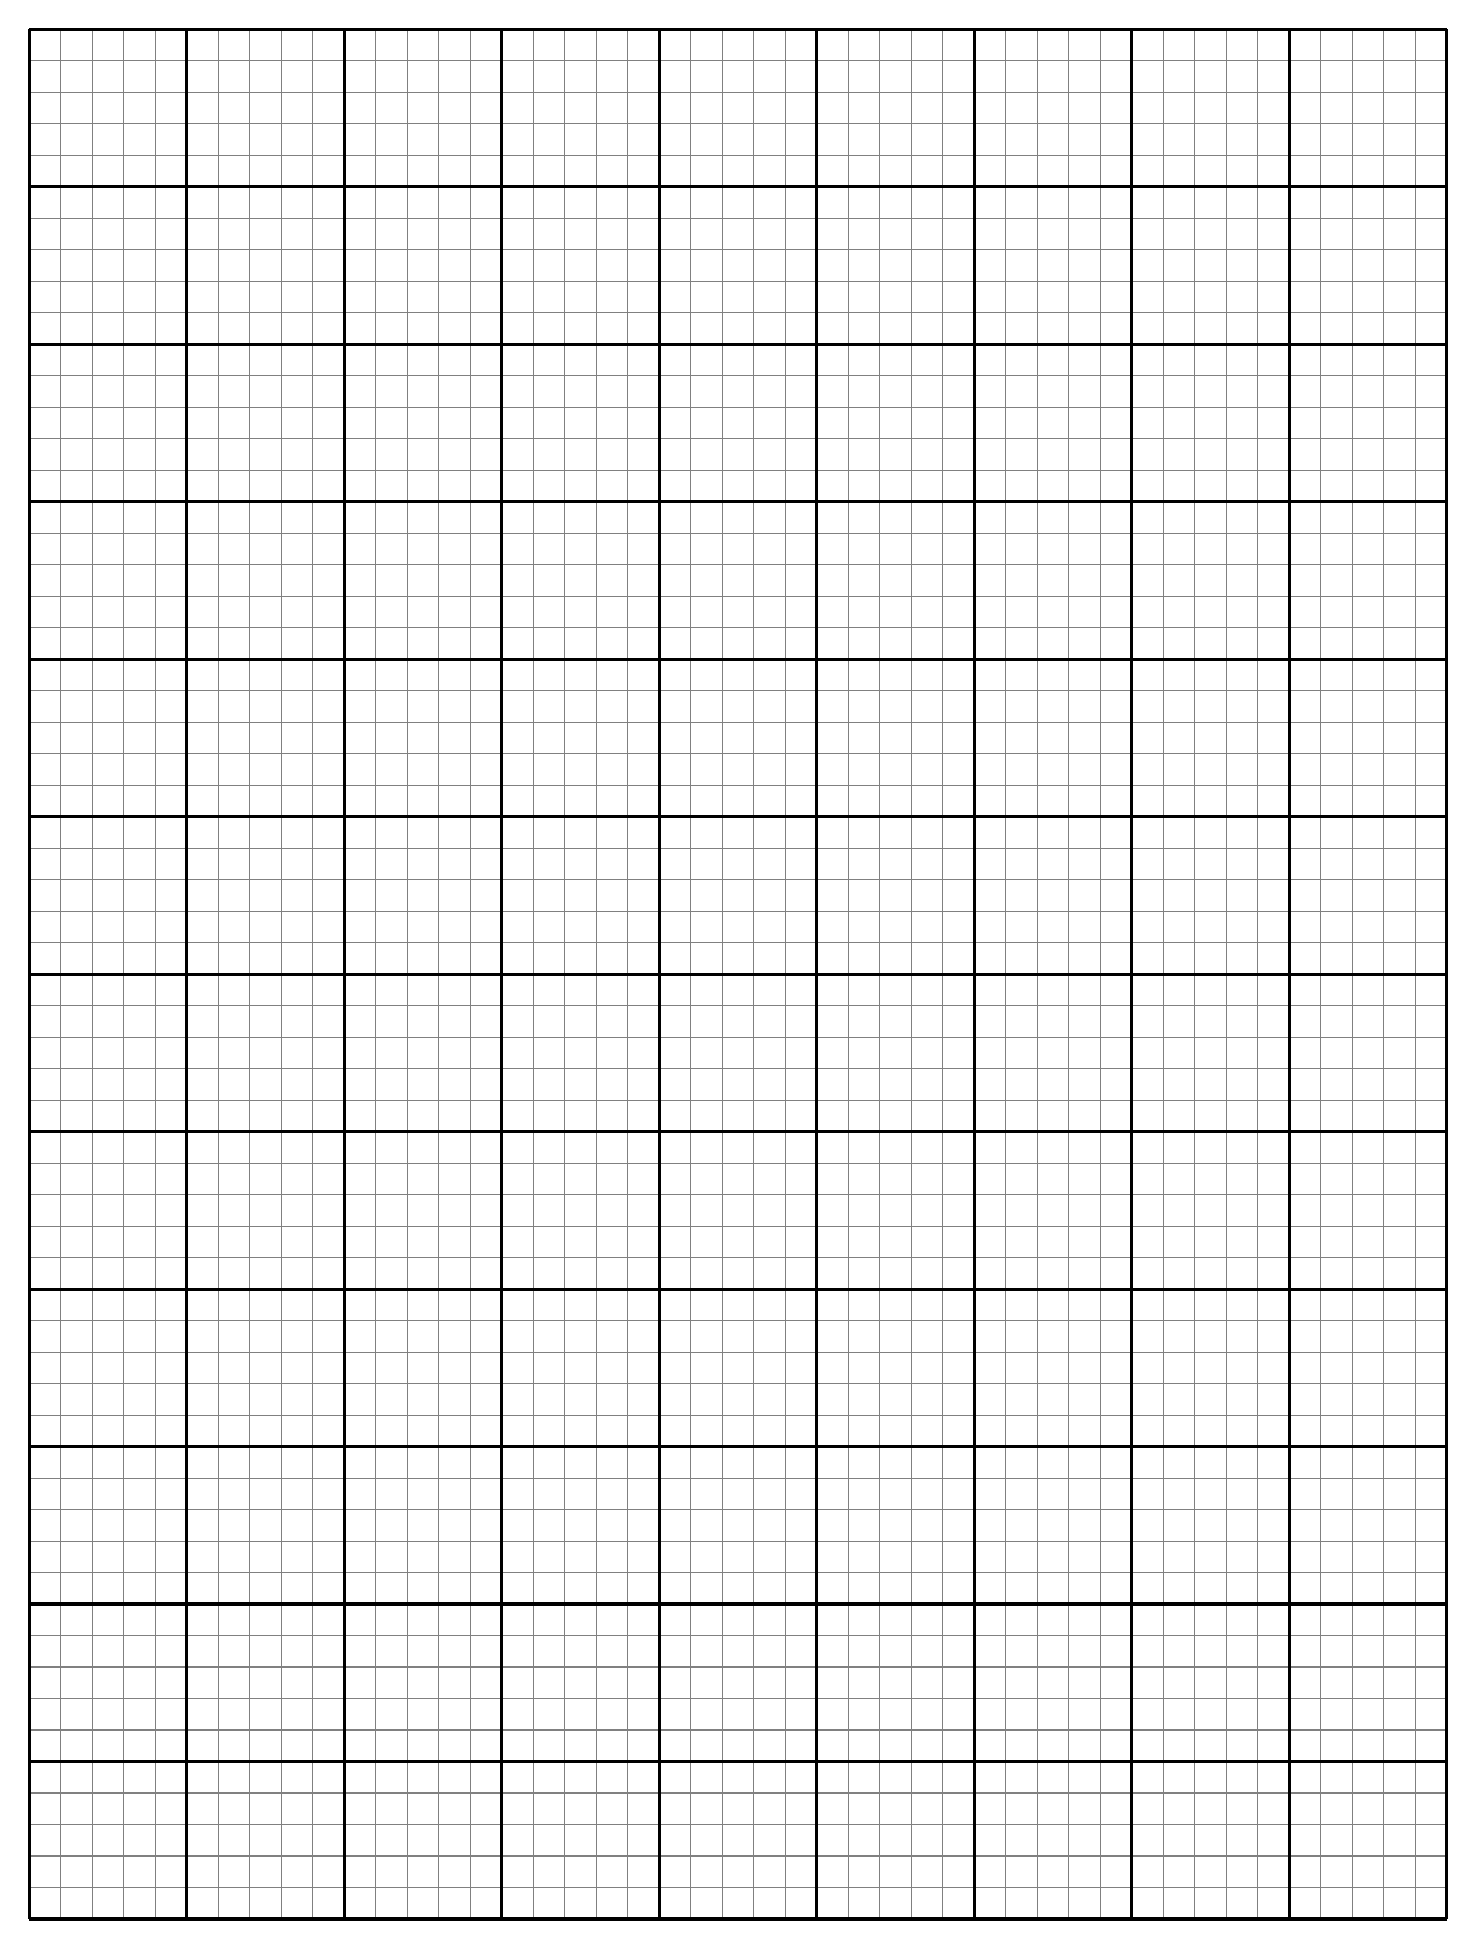
\begin{tikzpicture}[every node/.style={minimum size=1cm-\pgflinewidth, outer sep=10pt}, scale=2]
    \draw[step=0.2cm,color=gray] (0,0) grid (9,12);
    \draw[step=1cm,color=black,line width=0.4mm] (0,0) grid (9,12);
\end{tikzpicture}

\centering
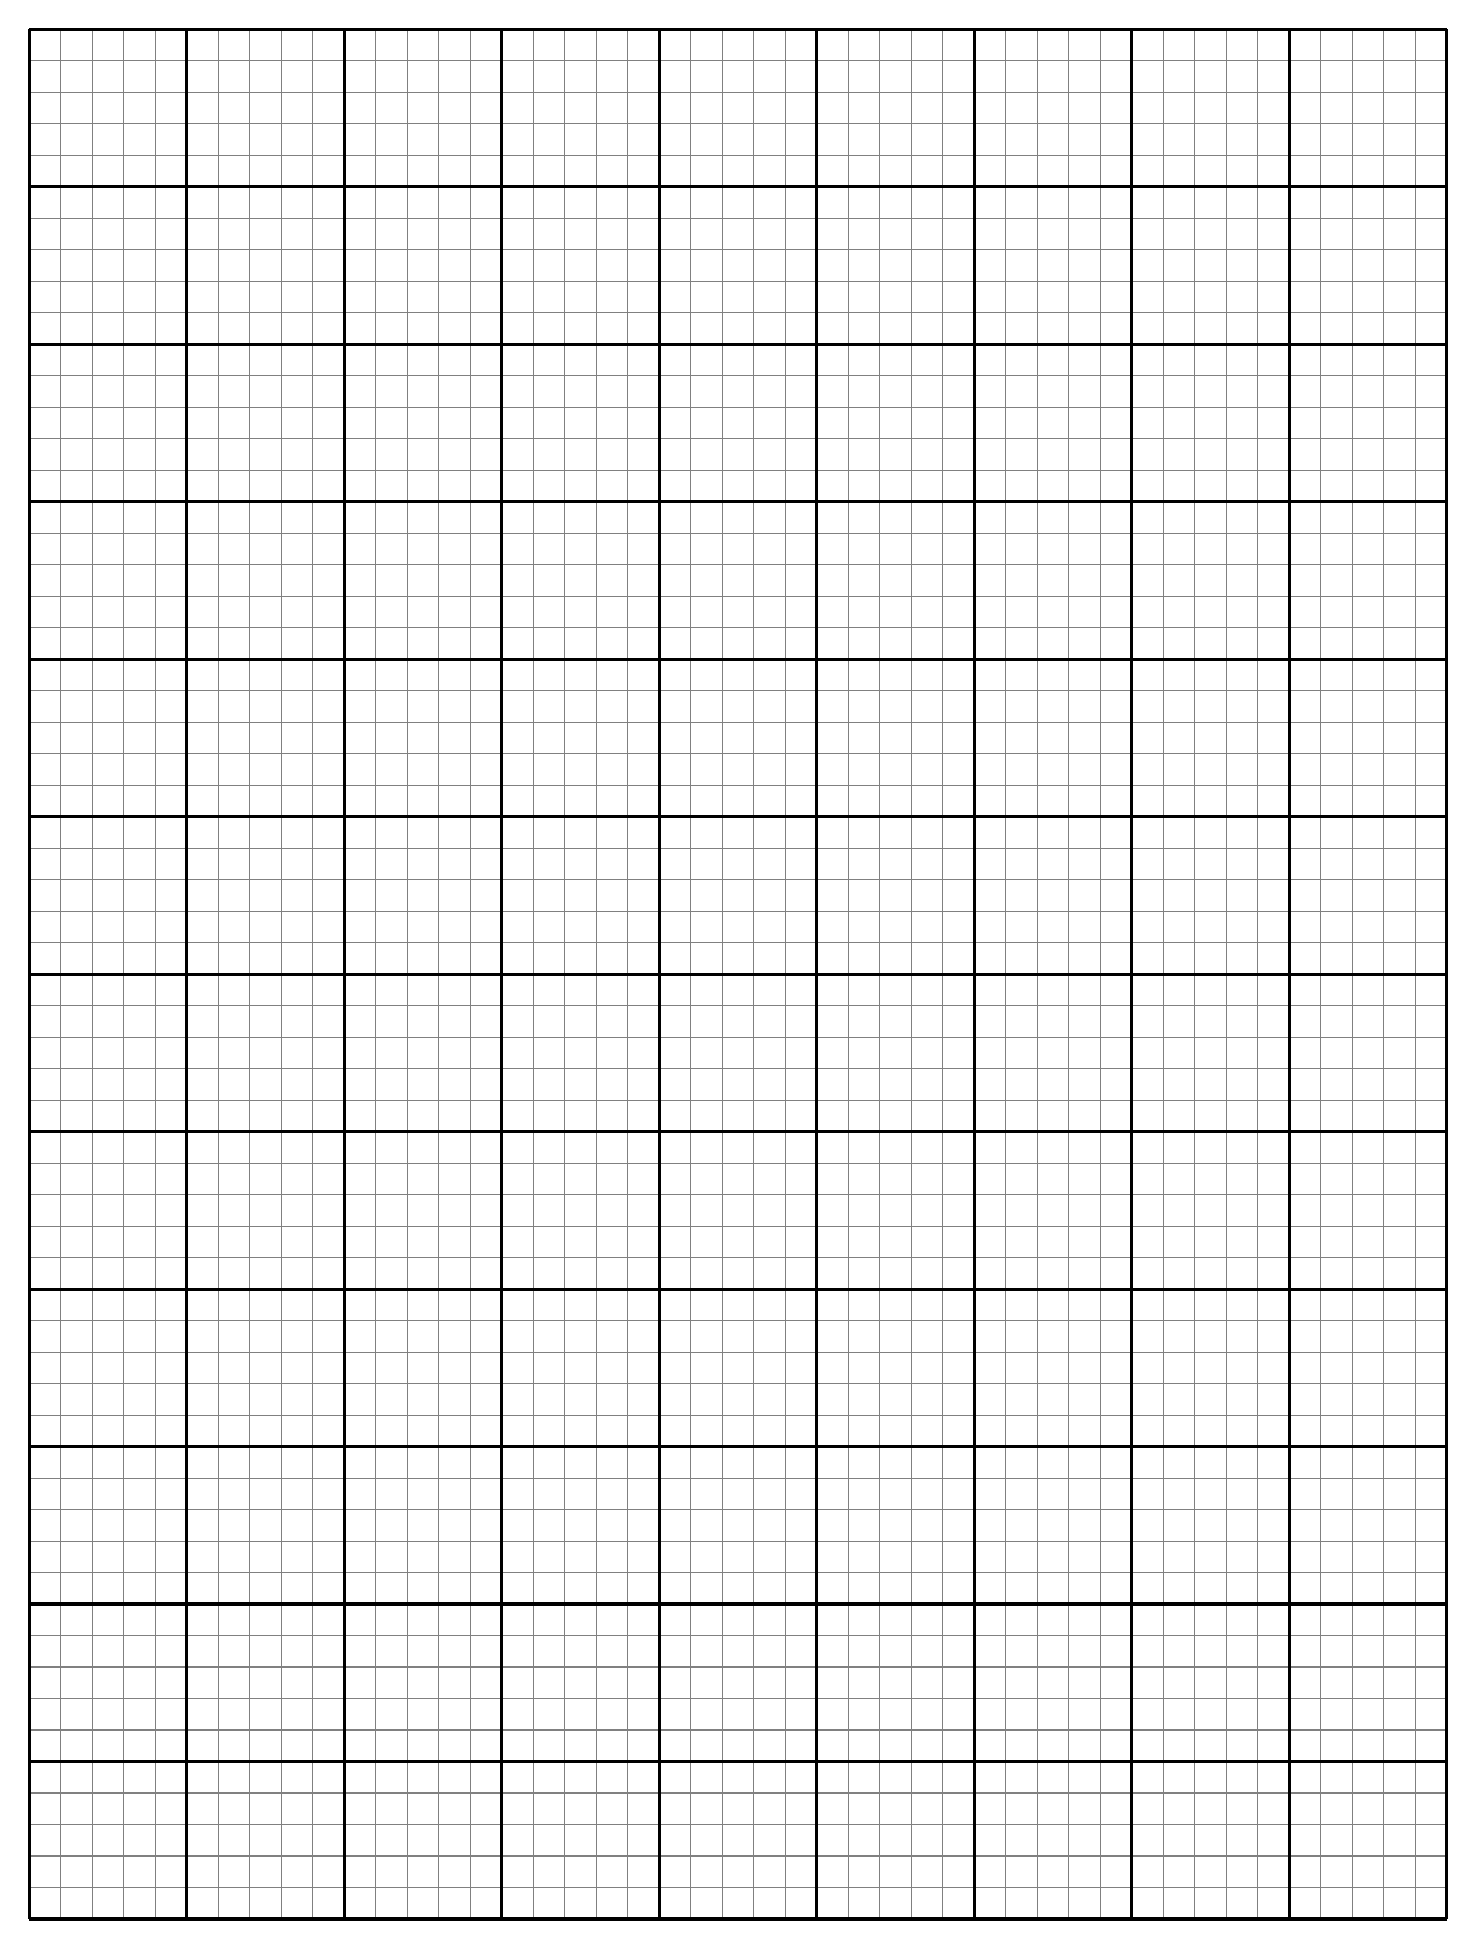
\begin{tikzpicture}[every node/.style={minimum size=1cm-\pgflinewidth, outer sep=10pt}, scale=2]
    \draw[step=0.2cm,color=gray] (0,0) grid (9,12);
    \draw[step=1cm,color=black,line width=0.4mm] (0,0) grid (9,12);
\end{tikzpicture}
\newpage
Empty
\newpage
Empty
\newpage
Empty